\documentclass[9pt,leqno]{beamer}
\usepackage{luatexja-otf}
\usepackage[T1]{fontenc}
\usepackage{textcomp}
\usepackage[utf8]{luainputenc}
\usepackage[noenc,safe]{tipa}
\usepackage{luatexja}
\usepackage{luatexja-ruby}
\usepackage[match]{luatexja-fontspec}
\usepackage[deluxe,hiragino-pron]{luatexja-preset}
\usepackage{etoolbox}
\usepackage{amsmath}
\usepackage{amssymb}
\usepackage{array}
\usepackage{hhline}
\usepackage{listings}
\usepackage{graphicx}
\usepackage{mathpazo}
\usepackage{pgfplots}
\usepackage{picture}
\usepackage{stmaryrd}
\usepackage{ulem}
\usepackage{wrapfig}
\usetheme{default}
\usefonttheme{professionalfonts}
\usecolortheme{seagull}
\setsansfont{Hiragino Kaku Gothic ProN W3}
\AtBeginEnvironment{quote}{\quotefont}
\newfontfamily{\quotefont}{Linux Biolinum O}
\renewcommand{\ttdefault}{lmtt}
\DeclareSymbolFont{letters}{OML}{ztmcm}{m}{it}
\DeclareSymbolFontAlphabet{\mathnormal}{letters}
\setbeamertemplate{navigation symbols}{}
\setbeamertemplate{items}[default]
\setbeamertemplate{caption}{\raggedright\insertcaption\par}
\renewcommand{\kanjifamilydefault}{\gtdefault}
\setbeamerfont{frametitle}{size=\large}
\setbeamerfont{caption}{size=\scriptsize}
\setbeamerfont{itemize/enumerate body}{size=\normalsize}
\setbeamerfont{itemize/enumerate subbody}{size=\normalsize}
\setbeamerfont{itemize/enumerate subsubbody}{size=\normalsize}
\DeclareMathOperator*{\argmax}{arg\,max}
\DeclareMathOperator*{\var}{var}
\renewcommand{\arraystretch}{1.2}
\newcommand{\q}[1]{“#1”}
\newcommand{\handwritten}[1]{\textit{\quotefont #1}}
\newcommand{\uprightquote}[1]{\normalfont{\quotefont #1}}
\newcommand{\thc}[1]{\multicolumn{1}{c}{#1}}
\hypersetup{%
    unicode,%
    colorlinks=true
}
\pgfplotsset{
    width=5cm,
    compat=newest,
    xlabel near ticks,
    ylabel near ticks
}
\title{{\huge \textbf{5} }Collocations}
\author{宮澤 彬}
\institute{総研大 宮尾研究室 博士前期\hbox{}1\hbox{}年}
\date{\today}
\begin{document}
\lstset{language=Python,basicstyle=\ttfamily\small}
\abovedisplayskip=2pt
\belowdisplayskip=5pt
\jot=3pt
{\usebackgroundtemplate{\includegraphics[width=5cm]{dice.pdf}}
%<a href="https://openclipart.org/pdf/people/casino/1391010041.svg">Dice (PDF)</a>
\begin{frame}
    \frametitle{{\small Foundations of Statistical Natural Language Processing 輪読会資料}}
    \titlepage
\end{frame}
}

\begin{frame}
    \begin{quote}
        Collocations of a given word are statements of the habitual or customary places of that word.

        \begin{flushright}
            John Rupert Firth
        \end{flushright}
        
        {\small ある語のコロケーションとは(個人の)習慣的あるいは(文化の)慣例的なその語の(置かれる)場所である.}
    \end{quote}


    \smallskip
    
    母語話者でないとなかなか分からない微妙な使い分け
    \begin{itemize}
        \item 「ご飯を炊く」と言うが「ほうれん草を炊く」とは言わない
        \item 「抹茶を点てる」や「風呂を点てる」などとは言うが
            
            「インスタントコーヒーを点てる」とは言わない
    \end{itemize}

    コロケーションは構成的でない.
    表現が構成的であるとは部分の意味から全体の意味を推測できること.

    不正確な表現ではあるが$\raise.6pt\hbox{$\llbracket \cdot \rrbracket$}$を『意味』とすれば
        \begin{align*}
            \llbracket \text{\uprightquote{sunny and warm}} \rrbracket = \llbracket \text{\uprightquote{sunny}} \rrbracket \land \llbracket \text{\uprightquote{warm}} \rrbracket
        \end{align*}
    のようなものは構成的で
        \begin{align*}
            \llbracket \lower.6pt\hbox{腹を立てる} \rrbracket \neq \llbracket \lower.6pt\hbox{立てる} \rrbracket(\llbracket \lower.6pt\hbox{腹} \rrbracket)
        \end{align*}
    のようなものは構成的でない.
\end{frame}
\begin{frame}
    \frametitle{5.1 Frequency}
    
    コロケーションを見つけるためにはコーパス中のNグラムで発生頻度が高いものを
    集めればよい.しかしNグラムの頻度を単純に数えると上位がほとんど \uprightquote{of the}, \uprightquote{in the} のような機能語の組み合わせ
    で占められてしまい,有用な情報が得られない.
    
    \bigskip

    これを解決する1つの方法は,特定の品詞の組み合わせのみを抽出することである.

    \begin{center}
        \begin{table}[h]
            \begin{tabular}{cl}
                \thc{Tag Pattern} & \thc{Example} \\
                \hline
                A N            & \uprightquote{commutative ring} \\
                N N            & \uprightquote{Banach space} \\
                A A N          & \uprightquote{stochastic differential equation} \\
                A N N          & \uprightquote{normed vector space} \\
                N A N          & \uprightquote{Jordan measurable set} \\
                N N N          & \uprightquote{probability density function} \\
                N P N          & \uprightquote{convergence in probability}
            \end{tabular}    
        \end{table}
    \end{center}

    \uprightquote{New York} や \uprightquote{United States} のような複合語が抽出されやすい.

\end{frame}

\begin{frame}
    \frametitle{5.1 Frequency}
    
    バイグラムの最初の単語を \uprightquote{strong} に限定したものと \uprightquote{powerful} に限定したものとを
    比較することでこれら2つの語の使い分けについて知ることができる.
    
    \begin{center}
        \begin{table}[h]
            \begin{tabular}{lclc}
                \thc{$w$} & \thc{$C(\text{\uprightquote{strong}},\, w)$} & \thc{$w$} & \thc{$C(\text{\uprightquote{powerful}},\, w)$}\\
                \hline
                \uprightquote{support}    & $50$ & \uprightquote{force}     & $13$ \\
                \uprightquote{safty}      & $22$ & \uprightquote{computers} & $10$ \\
                \uprightquote{sales}      & $21$ & \uprightquote{position}  &  $8$ \\
                \uprightquote{opposition} & $19$ & \uprightquote{men}       &  $8$ \\
                \uprightquote{showing}    & $18$ & \uprightquote{computer}  &  $8$ \\
                \uprightquote{sense}      & $18$ & \uprightquote{man}       &  $7$ \\
            \end{tabular}    
        \end{table}
    \end{center}

    英作文で使いたい動詞と一緒に使うべき前置詞
    が分からないとき,いくつかの適当な前置詞と組み合わせたものを
    Googleで検索して,そのヒット件数で正解を決めることと似ている.

\end{frame}

\begin{frame}
    \frametitle{5.2 Mean and Variance}

    語の共起は連続しているとは限らず,
    Nグラムの頻度をただ数えるだけでは不十分である.

    \smallskip

    \begin{itemize}
        \item[\uprightquote{(a)}] \uprightquote{she \textbf{knocked} on his \textbf{door}}

        \item[\uprightquote{(b)}] \uprightquote{they \textbf{knocked} at the \textbf{door}}
            
        \item[\uprightquote{(c)}] \uprightquote{100 women \textbf{knocked} on Donaldson's \textbf{door}}
          
        \item[\uprightquote{(d)}] \uprightquote{a man \textbf{knocked} on the metal front \textbf{door}}
    \end{itemize}
    \ltjsetparameter{autoxspacing=true}

    \smallskip

    しかし,規則性がないわけではない.
    実際このような文脈で \uprightquote{knocked} の代わりに \uprightquote{hit} や \uprightquote{beat} は普通使わない.
    
\end{frame}

\begin{frame}
    \frametitle{5.2 Mean and Variance}
    離れた位置にあるコロケーションを扱うために,各単語の前後の $N$ 個(通常 $N=3$ または $N=4$)の単語で組を作る.
    こうして得られたすべてのバイグラムを通常バイグラムと同様に扱えばよい.

    \bigskip

    \begin{center}
        \uprightquote{Sentence: }\handwritten{Stocks crash as rescue plan teeters}
    \end{center}
    \begin{center}
        \begin{table}[h]
            \begin{tabular}{l|l|l|l|l}
                \handwritten{stocks crash} & \handwritten{stocks as} & \handwritten{stocks rescue} &                            &   \\
                                           & \handwritten{crash as}  & \handwritten{crash rescue}  & \handwritten{crash plan}  &   \\
                                           &                          & \handwritten{as rescue}     & \handwritten{as plan}     & \handwritten{as teeters} \\
                                           &                          &                              & \handwritten{rescue plan} & \handwritten{plan teeters} 
            \end{tabular}    
        \end{table}
    \end{center}
\end{frame}

\begin{frame}
    \frametitle{5.2 Mean and Variance}
    \uprightquote{knocked} と \uprightquote{door} の関係を知る方法として,2語の符号付き距離の平均と分散を求める方法がある.
    前頁の例文(a)-(d)で \uprightquote{knocked} から \uprightquote{door} までの符号付き距離(\uprightquote{door} が \uprightquote{knocked}の後ろにあるときを正,前にあるときを負とする)の
    標本平均を計算すると
    \begin{align*}
        \frac{1}{4}(3 + 3 + 5 + 5) = 4
    \end{align*}
    である.
    %\uwave{母集団が平均$\mu$の正規分布に従っているならば}
    %\begin{align*}
    %    \frac{\overline{x} - \mu}{s / \sqrt{N}} \sim t(N - 1)
    %\end{align*}
    %が成り立つ.
    また標本分散は
    \begin{align*}
        s^2 &= \frac{1}{N - 1}\sum_{i = 1}^N \left(d_i - \overline{d}\right)^2 \\
            &= \frac{1}{3}\left((3 - 4)^2 + (3 - 4)^2 + (5 - 4)^2 + (5 - 4)^2\right) = \frac{4}{3}
    \end{align*}
    であるが,コロケーションに関する評価では慣例的に標準偏差を用いるので,これを計算して
    \begin{align*}
        s = \frac{2}{\sqrt{3}} \approx 1.15
    \end{align*}
    を得る.
\end{frame}


\begin{frame}
    \frametitle{5.2 Mean and Variance}
    このようにして得られた平均と標準偏差をどのように解釈するか?
    \begin{itemize}
        \item 平均が $1$ に近く,標準偏差が $0$ に近い
            \begin{itemize}
                \item 連続した2語として現れやすい
                    
                \uprightquote{New, York} $\left(\overline{d} = 0.97,\, s = 0.43\right)$
            \end{itemize}
        \item 平均が $1$ よりもずっと大きく,標準偏差が $0$ に近い
            \begin{itemize}
                \item 間隔を空けて使われる表現が定型化している
                    
                    \uprightquote{previous, games} $\left(\overline{d} = 1.83,\, s = 0.48\right)$ $\to$ \uprightquote{privious $N$ games}
            \end{itemize}

        \item 平均が $0$ に近く,標準偏差が大きい
            \begin{itemize}
                \item あまり関連がない

                \uprightquote{editorial, Atlanta} $\left(\overline{d} = 0.44,\, s= 4.03\right)$
            \end{itemize}
    \end{itemize}
\end{frame}

%histogram
\begin{frame}
    \frametitle{5.2 Mean and Variance}
    度数分布図を描くと直感的に分かりやすい.
    \begin{center}
        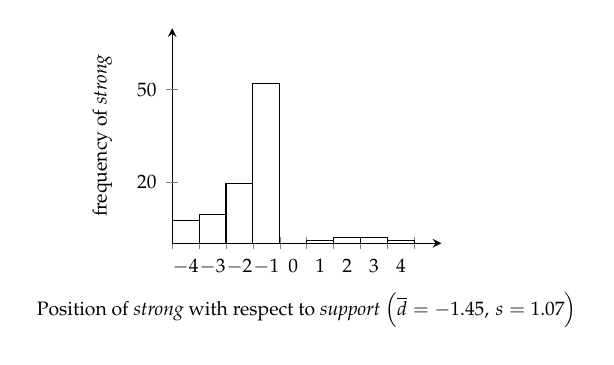
\begin{tikzpicture}[font=\scriptsize]
            \begin{axis}[
                ybar,
                bar width=10pt,
                xlabel={\uprightquote{Position of \textit{strong} with respect to \textit{support} $\left(\overline{d} = -1.45,\, s = 1.07\right)$}},
                ylabel={\uprightquote{frequency of \textit{strong}}},
                ymin=0, ymax=70,
                xmax=6,
                ytick=\empty, extra y ticks={20, 50},
                xtick=data, x tick label as interval=true,
                axis x line=bottom,
                axis y line=left
            ]
            \addplot[
                ybar interval,
                fill=white
            ]
            coordinates {
                (-4,7.5)
                (-3,9.5)
                (-2,19.5)
                (-1,52)
                (0,0)
                (1,1)
                (2,2)
                (3,2)
                (4,1)
                (5,0)
            };
            \end{axis}
        \end{tikzpicture}

        \bigskip

        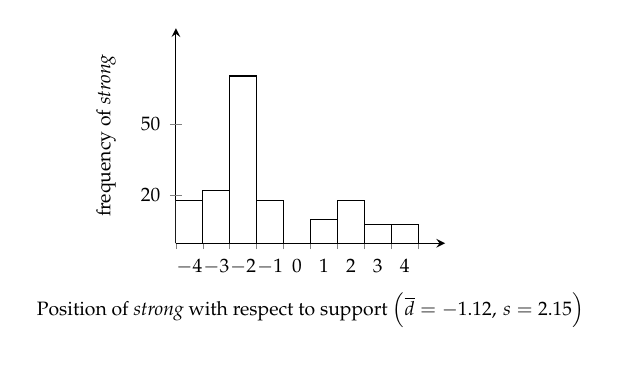
\begin{tikzpicture}[font=\scriptsize]
            \begin{axis}[
                ybar,
                bar width=10pt,
                xlabel={{\uprightquote Position of \textit{strong} with respect to {\uprightquote support} $\left(\overline{d} = -1.12,\, s = 2.15\right)$}},
                ylabel={{\uprightquote frequency of \textit{strong}}},
                ymin=0,
                ymax=90,
                xmax=6,
                ytick=\empty,
                extra y ticks={20, 50},
                xtick=data,
                x tick label as interval=true,
                axis x line=bottom,
                axis y line=left
            ]
            \addplot[
                ybar interval,
                fill=white
            ]
            coordinates {
                (-4,18)
                (-3,22)
                (-2,70)
                (-1,18)
                (0,0)
                (1,10)
                (2,18)
                (3,8)
                (4,8)
                (5,0)
            };
            \end{axis}
        \end{tikzpicture}
    \end{center}
\end{frame}

\begin{frame}
    \frametitle{5.3 Hypothesis Testing}
    頻度が多い単語2語の組み合わせを多く見つけた場合,
    他の組み合わせと比較して多いかどうかが知りたい.
    そこでコロケーションについて検定を行うことにする.

    \bigskip

    検定のため簡単なモデルを考える.
    トークン1つを1回の試行とし,特定の語 $w$ の出現を成功と捉えるBernoulli試行とみなす.
    $N$ 個のトークン(つまり $N$ 回の試行)のうちに $w$ が $n$ 回出現するとする.
    Bernoulli分布のパラメータ $p$ の最尤推定量 $P(w)$ は
    \begin{align*}
            \argmax_{\vartheta \in (0,1)}\left(\log \vartheta^n(1 - \vartheta)^{N - n}\right) = \frac{n}{N}
    \end{align*}
    で求められるから,例えばp. 166にデータが示されている \uprightquote{unsalted} と \uprightquote{butter} の
    出現する確率は
    \begin{align*}
        P(\text{\uprightquote{unsalted}}) = \frac{20}{14307668}\,, \quad P(\text{\uprightquote{butter}}) = \frac{320}{14307668}
    \end{align*}
    であると考えられる.

\end{frame}

\begin{frame}
    \frametitle{5.3 Hypothesis Testing}
    興味があるのはこれらが共起する場合である.
    そこで$N$ 個のトークンの列を $N$ 個のバイグラムの並び(文頭または文末のどちらか一方だけに特殊な記号を追加?)と捉えて,
    各バイグラムを1回の試行とし,特定のバイグラムの出現を成功とする Bernoulli 試行とみなす.
    これらの出現が独立であるという帰無仮説を立てて検定を行う.
    
    \begin{align*}
        H_0 \,:\, P(\text{\uprightquote{unsalted butter}}) = P(\text{\uprightquote{unsalted}}) P(\text{\uprightquote{butter}})
    \end{align*}

    \bigskip

    $H_0$ が正しいならば,$i$ 回目の結果を表す確率変数を $X_i:\varOmega \to \{0,\,1\}$ としたとき
    \begin{align*}
        X_1,\,\ldots,\,X_N \stackrel{\mathrm{i.i.d.}}{\mbox{\scalebox{3}[1]{$\sim$}}}
        \mathrm{Bern}\left(p := P(\text{\uprightquote{unsalted}}) P(\text{\uprightquote{butter}})\right)
    \end{align*}
    である.$N$ が大きいので de Moivre Laplace の定理により
    \begin{align*}
        Z := \frac{\sum_{i = 1}^N X_i - Np}{\sqrt{Np(1-p)}}
        %= \frac{\overline{X} - p}{\sqrt{p(1-p)}/\sqrt{N}} 
        \stackrel{\mathrm{approx.}}{\mbox{\scalebox{4}[1]{$\sim$}}} \mathcal{N}(0,1)
    \end{align*}
    が成り立つから,以下では $Z \sim \mathcal{N}(0,1)$ として検定を行う.
\end{frame}

\begin{frame}[fragile]
    \frametitle{5.3.1 The t test}
    $p$ が $0$ に近いので $p(1 - p) \simeq p$ が成り立つ.ゆえに観測値を $x_1,\,\ldots,\,x_n$ とすると
    \begin{align*}
        Z \simeq \frac{\sum_{i = 1}^N x_i - Np}{\sqrt{Np}} = \frac{20 - 24 \cdot 320 / 14307668}{\sqrt{24 \cdot 320 /14307668}}
        \approx 863
    \end{align*}
    となる.以下の計算により $H_0$ は有意水準1\%で棄却される.
    したがって\uprightquote{unsalted butter}はコロケーションであるといえる.

    \bigskip
    \begin{lstlisting}
    >>> import scipy.stats
    >>> scipy.stats.norm.cdf(863)
    1.0
    \end{lstlisting}
    \begin{center}
        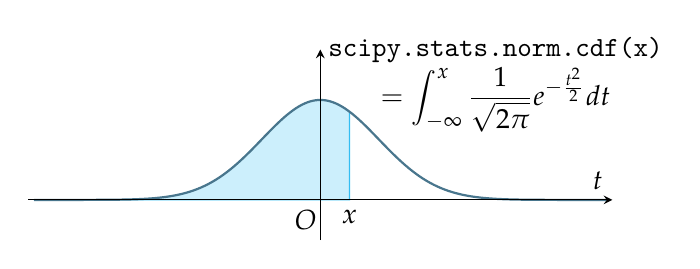
\begin{tikzpicture}[
            declare function={
                gauss(\x,\mu,\sigma)=(1/(\sigma * sqrt(2 * pi))) * exp(-((\x-\mu)^2/(2*\sigma^2));
            }
        ]
            \begin{axis}[
                  axis lines=middle,
                  axis on top,
                  domain=-4.9:4.9, 
                  samples=200,
                  xlabel={$t$},
                  ylabel=\empty,
                  height=4cm, width=9cm,
                  xmin=-5, xmax=5,
                  ymin=-0.4, ymax=1.5,
                  xtick=\empty,
                  %xticklabel style={xshift=5},
                  ytick=\empty,
                  enlargelimits=false, 
                  clip=false
              ]
              \addplot [fill=cyan!20, draw=cyan!80, domain=-4.9:0.5] {2.5 * gauss(x,0,1)} \closedcycle;
              \addplot [thick, cyan!50!black] {2.5 * gauss(x,0,1)};
              \draw (3,1.5) node {\texttt{scipy.stats.norm.cdf(x)}};
              %\draw (3,1.5) node {$\mathtt{scipy.stats.norm.cdf(x)}$}; '()' が roman になる
              \draw (3,1) node {$\displaystyle =\int_{-\infty}^{x} \frac{1}{\sqrt{2\pi}}e^{-\frac{t^2}{2}}dt$};
              \draw (-0.25,0) node[below] {$O$};
              \draw (0.5,0) node[below] {$x$};
            \end{axis}
        \end{tikzpicture}
    \end{center}
\end{frame}

\begin{frame}
    \frametitle{5.3.1 The t test}
    教科書では $t$ 値を用いて検定を行なっているが,
    \begin{itemize}
        \item $X_1,\,\ldots,\,X_N$ がそれぞれ独立に同一の正規分布に従う.
        \item 母分散 $\sigma^2$ が未知である.
    \end{itemize}
    が成立していないので $t$ 値を使うのは不適当である.

    \smallskip
    
    しかし
    \begin{quote}
        When the expected cooccurrence frequency $E_{11}$ (under $H_0$) is small, z-score values can become very large,
        leading to highly inflated scores for low-frequency pair types.
        The cause of this problem can be traced back to the denominator of the z-score equation,
        where $E_{11}$ is the (approximate) variance of $\,X_{11}$ under the point null hypothesis of independence.    
        \begin{flushright}
            \normalfont{\texttt{\href{http://www.collocations.de/AM/section4.html}{http://www.collocations.de/AM/section4.html}}}
        \end{flushright}
    \end{quote}

    さらに
    \begin{quote}
        The t test and other statistical tests are most useful as
        a method for ranking collocations. The level of significance itself is less
        useful. In fact, in most publications that we cite in this chapter, the level
        of significance is never looked at. All that is used is the scores and the
        resulting ranking.
        \begin{flushright}
            Foundations of Statistical Natural Language Processing p. 166
        \end{flushright}
    \end{quote}
\end{frame}

\begin{frame}
    \frametitle{5.3.2 Hypothesis testing of differences}
    母集団の平均の差に関する検定(量)により,似たような意味を持つ2つの語の使い分けについて知ることができる.
    $\mathcal{N}(\mu_x, \sigma_x^2)$ に従う母集団からの大きさ $N_x$ の標本平均を $\overline{X}$,
    $\mathcal{N}(\mu_y, \sigma_y^2)$ に従う母集団からの大きさ $N_y$ の標本平均を $\overline{Y}$ とする.
    正規分布の重ね合わせの性質より,
    \begin{align*}
        Z := \frac{\left(\overline{X} - \overline{Y}\right) - \left(\mu_x - \mu_y \right)}{{\displaystyle \sqrt{\frac{\sigma_x^2}{N_x} + \frac{\sigma_y^2}{N_y}}}} \sim \mathcal{N}(0,\,1)
    \end{align*}
    が成り立つ.帰無仮説を
    \begin{align*}
        H_0 \,:\, \mu_x = \mu_y
    \end{align*}
    として検定を行いたいところであるが,前頁で見たように検定にはあまり興味がない.知りたいのは $\mu_x = \mu_y$ のときの $Z$ である.
    今回の設定では,比較したい(似ている)単語を$v^1$, $v^2$ とし,それ以外の各単語 $w$ について
    \begin{align*}
        Z \simeq \frac{P\left(v^1 w\right) - P\left(v^2 w\right)}{{\displaystyle \sqrt{\frac{P\left(v^1 w\right)}{N_x} + \frac{P\left(v^2 w\right)}{N_y}}}}
        = \frac{C\left(v^1 w\right) - C\left(v^2 w\right)}{\sqrt{C\left(v^1 w\right) + C\left(v^2 w\right)}}
    \end{align*}
    を計算する.ここでは $N_x = N_y$ であることを使った.

\end{frame}

\begin{frame}
    \frametitle{5.3.2 Hypothesis testing of differences}
    \begin{center}
        \begin{table}
            \begin{tabular}{rrrrl}
                \thc{$Z$}& \thc{$C(w)$} & \thc{$C(\text{\uprightquote{strong }}w)$}& \thc{$C(\text{\uprightquote{powerful }} w)$} & \thc{$w$} \\
                \hline
                $-3.1622$ &  $933$ &  $0$ & $10$ & \uwave{\uprightquote{computers}}\\
                $-2.8284$ & $2337$ &  $0$ &  $8$ & \uprightquote{computer}\\
                $-2.4494$ &  $289$ &  $0$ &  $6$ & \uprightquote{symbol}\\
                $-2.4494$ &  $588$ &  $0$ &  $6$ & \uprightquote{machines}\\
                $-2.2360$ & $2266$ &  $0$ &  $5$ & \uprightquote{Germany}\\
                \multicolumn{5}{c}{$\vdots$}\\
                $4.0249$  & $1093$ & $19$ &  $1$ & \uprightquote{opposition} \\
                $4.5825$  & $3741$ & $21$ &  $0$ & \uprightquote{sales}\\
                $4.6904$  &  $986$ & $22$ &  $0$ & \uprightquote{safety}\\
                $6.3257$  & $3616$ & $58$ &  $7$ & \uprightquote{enough}\\
                $7.0710$  & $3685$ & $50$ &  $0$ & \uwave{\uprightquote{support}}
            \end{tabular}
        \end{table}
    \end{center}
    このランキングから\uprightquote{powerful}が\uprightquote{computer}のような実体のあるものの強さを表し,
    \uprightquote{strong}が\uprightquote{support}のような内面的な強さを表している傾向をつかむことができる.
\end{frame}
\begin{frame}
    \frametitle{5.3.3 Pearson$\text{\CID{96}}$s chi-square test}
    $t$ 検定が使えるのは母集団が正規分布していると
    仮定できる場合のみである.しかし実際のところ,
    普通はそのように仮定することができない.
    代替手段として分割表を用いた独立性の検定を
    コロケーションかどうかの判定に使うことを考える.

    \smallskip

    {\small 教科書で用いられている公式 (5.7) の導出}

    {\fontsize{6pt}{7.2}\selectfont
    \begin{table}
        \begin{center}
            \begin{tabular}{|c|c|c|c|}
                \hline
                          & $X$     & $\lnot X$ &     \\
                \hline
                $Y$       & $a$     & $b$       & $a + b$\\
                \hline
                $\lnot Y$ & $c$     & $d$       & $c + d$\\
                \hline
                          & $a + c$ & $b + d$   & $a + b + c + d$ \\
                \hline
            \end{tabular}
        \end{center}
    \end{table}
    }
    {\fontsize{6pt}{7.2}\selectfont
    \begin{align*}
        \chi^2 &:= \dfrac{\left(a - \dfrac{(a + b)(a + c)}{a + b + c + d}\right)^2}{\dfrac{(a + b)(a + c)}{a + b + c + d}}
                   + \dfrac{\left(b - \dfrac{(a + b)(b + d)}{a + b + c + d}\right)^2}{\dfrac{(a + b)(b + d)}{a + b + c + d}}
                   + \dfrac{\left(c - \dfrac{(c + d)(a + c)}{a + b + c + d}\right)^2}{\dfrac{(c + d)(a + c)}{a + b + c + d}}
                   + \dfrac{\left(d - \dfrac{(c + d)(b + d)}{a + b + c + d}\right)^2}{\dfrac{(b + d)(a + c)}{a + b + c + d}}\\
                   &\phantom{:}= \dfrac{\dfrac{(ad - bc)^2}{(a + b + c + d)^2}}{\dfrac{(a + b)(a + c)}{a + b + c + d}}
                   + \dfrac{\dfrac{(ad - bc)^2}{(a + b + c + d)^2}}{\dfrac{(a + b)(b + d)}{a + b + c + d}}
                   + \dfrac{\dfrac{(ad - bc)^2}{(a + b + c + d)^2}}{\dfrac{(c + d)(a + c)}{a + b + c + d}}
                   + \dfrac{\dfrac{(ad - bc)^2}{(a + b + c + d)^2}}{\dfrac{(b + d)(a + c)}{a + b + c + d}}\\
                   &\phantom{:}= \frac{(ad - bc)^2\left((c + d)(b + d) + (c + d)(a + c) + (a + b)(b + d) + (a + b)(c + d)\right)}{(a + b + c + d)(a + b)(c + d)(a + c)(b + d)} \\
                   &\phantom{:}= \frac{(a + b + c + d)(ad - bc)^2}{(a + b)(c + d)(a + c)(b + d)}
    \end{align*}
    }
\end{frame}


\begin{frame}[fragile]
    \frametitle{5.3.3 Pearson$\text{\CID{96}}$s chi-square test}
    帰無仮説として
    \begin{align*}
       H_0 \,:\, \text{\uprightquote{unsalted}と\uprightquote{butter}の出現は独立である.}
    \end{align*}
    を設定する.
    \begin{table}
        \begin{tabular}{|c|r|r|r|}
            \hline
            & \multicolumn{1}{c|}{\text{\uprightquote{unsalted}}} & \multicolumn{1}{c|}{$\lnot\text{\uprightquote{unsalted}}$} &     \\
            \hline
            \text{\uprightquote{butter}}        &            $20$                &               $300$        &  $320$\\
            \hline
            $\lnot\text{\uprightquote{butter}}$ &            $4$                 &          $14307344$        &  $14307348$\\
            \hline
                                                &            $24$                &          $14307644$        &  $14307668$\\
            \hline
        \end{tabular}
    \end{table}
    \begin{align*}
        \chi^2 = \frac{14307668(20 \cdot 14307344 - 300 \cdot 4)^2}{320 \cdot 14307348 \cdot 14307644 \cdot 24} \approx 745169
    \end{align*}
    
    \smallskip

    $\chi^2$ が $\mathrm{df} = (2 - 1)(2 - 1)=1$ の $\chi^2$ 分布における片側1\%点 $6.63$
    よりも大きいので,$H_0$ は棄却される.
    つまり\uprightquote{unsalted}と\uprightquote{butter}の
    出現は独立とはいえず,したがって\uprightquote{unsalted butter}はコロケーションであるといえる.

\end{frame}

\begin{frame}[fragile]
    \frametitle{5.3.3 Pearson$\text{\CID{96}}$s chi-square test}
    \begin{lstlisting}   
>>> import numpy as np
>>> import scipy.stats
>>> chi2, p, dof, expected = \
        scipy.stats.chi2_contingency(np.array(
        [[20,300],[4,14307344]]),correction=False)
>>> chi2, p, dof
(745168.95831120119, 0.0, 1)
    \end{lstlisting}
    \begin{center}
        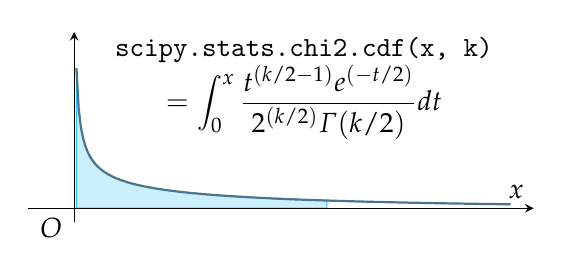
\begin{tikzpicture}[
            declare function={
                chi2(\x)=(1/(sqrt(2 * pi)) * (1/sqrt(\x)) * exp(-\x/2);
            }
            ]
            \begin{axis}[
                  axis lines=middle,
                  axis on top,
                  domain=-0.2:2, 
                  samples=200,
                  xlabel={$x$},
                  ylabel=\empty,
                  height=4cm, width=8cm,
                  xmin=-0.2, xmax=2,
                  ymin=-0.4, ymax=5,
                  xtick=\empty,
                  ytick=\empty,
                  clip=false
              ]
              \addplot [fill=cyan!20, draw=cyan!80, domain=0.01:1.1] {chi2(x)} \closedcycle;
              \addplot [thick, cyan!50!black, domain=0.01:1.9] {chi2(x)};
              \draw (1,4.5) node {\texttt{scipy.stats.chi2.cdf(x, k)}};
              \draw (1,3) node {${\displaystyle =\int_{0}^{x} \frac{t^{(k/2 - 1)}e^{(-t/2)}}{2^{(k / 2)} \varGamma(k/2)}dt}$};
              \draw (-0.1,0) node[below] {$O$};
            \end{axis}
        \end{tikzpicture}
    \end{center}

\bigskip

カイ二乗検定(量)のコロケーション以外の応用として,
コーパスの類似度の計測や,対訳コーパスの中の訳語の発見などがある.
\end{frame}

\begin{frame}
    \frametitle{5.3.4 Likelihood ratios}
    疎なデータに対してはカイ二乗検定より,
    尤度比を使ったほうがよい(Dunning 1993).
    \begin{table}
        \begin{tabular}{|c|c|c|c|}
            \hline
                          &    $w_2$       &  $\lnot w_2$                                      &   \\
            \hline
            $w_1$         &   $c_{12}$     & $c_1 - c_{12}$                                    &   $c_1$ \\
            \hline
            $\lnot{w_1}$  & $c_2 - c_{12}$ & $\left(N -c_1\right) - \left(c_2 - c_{12}\right)$ &  $N - c_1$ \\
            \hline
                          &     $c_2$      &     $c_2$                                         &    $N$ \\
            \hline
        \end{tabular}
    \end{table}
    $p_1 := P(w_2 | w_1)$,$p_2 := P(w_2 | \lnot w_1)$ とするとき,
    \begin{align*}
        H_1 \,:\, p_1 = p_2\,,\quad H_2 \,:\, p_1 \neq p_2
    \end{align*}
    という仮説を立てる.
    
    $H_2$ が正しいと仮定したとき最尤推定量は
    \begin{align*}
        L(H_2) &:= \binom{c_1}{c_{12}}p_1^{c_{12}}(1 - p_1)^{c_1 - c_{12}}
        \binom{ N - c_1}{c_2 - c_{12}}p_2^{c_2 - c_{12}}(1 - p_2)^{(N - c_1) - (c_2 - c_{12})} \\
        & \phantom{:} = \binom{c_1}{c_{12}}\left(\frac{c_{12}}{c_1}\right)^{c_{12}}\left(1 - \frac{c_{12}}{c_1}\right)^{c_1 - c_{12}} \\
        & \qquad \qquad \binom{ N - c_1}{c_2 - c_{12}}\left(\frac{c_2 - c_{12}}{N - c_1}\right)^{c_2 - c_{12}}\left(1 - \frac{c_2 - c_{12}}{N - c_1}\right)^{(N - c_1) - (c_2 - c_{12})}
    \end{align*}
    である.
\end{frame}
\begin{frame}   
    \frametitle{5.3.4 Likelihood ratios}
    一方 $H_1$ が正しいと仮定したとき最尤推定量は
    \begin{align*}
        L(H_1) &:= \binom{c_1}{c_{12}}p^{c_{12}}(1 - p)^{c_1 - c_{12}}
        \binom{ N - c_1}{c_2 - c_{12}}p^{c_2 - c_{12}}(1 - p)^{(N - c_1) - (c_2 - c_{12})} \\
        &\phantom{:}= \binom{c_1}{c_{12}}\left(\frac{c_2}{N}\right)^{c_{12}}\left(1 - \frac{c_2}{N}\right)^{c_1 - c_{12}} \\
        & \qquad \qquad \binom{ N - c_1}{c_2 - c_{12}}\left(\frac{c_2}{N}\right)^{c_2 - c_{12}}\left(1 - \frac{c_2}{N}\right)^{(N - c_1) - (c_2 - c_{12})}
    \end{align*}
    である.

    $H_1$ と $H_2$ の尤度比を $\lambda := L(H_1) / L(H_2)$ とすると,
    $-2 \log \lambda$ は漸近的に自由度1のカイ二乗分布に従うことが知られている.
    $-2 \log \lambda$ は $H_2$ が尤もらしいとき大きい値をとる.
    
\end{frame}

\begin{frame}
    \frametitle{5.3.4 Likelihood ratios}
    \begin{center}
        \begin{table}
            \begin{tabular}{rrrrll}
                \thc{$-2 \log \lambda$}& \thc{$C(w^1)$} & \thc{$C(w^2)$}& \thc{$C(w^1w^1)$} & \thc{$w^1$} & \thc{$w^2$}\\
                \hline
                $-3.1622$ &  $933$ &  $0$ & $10$ & \uwave{\uprightquote{computers}} & \\
                $-2.8284$ & $2337$ &  $0$ &  $8$ & \uprightquote{computer} & \\
                $-2.4494$ &  $289$ &  $0$ &  $6$ & \uprightquote{symbol} & \\
                $-2.4494$ &  $588$ &  $0$ &  $6$ & \uprightquote{machines} & \\
                $-2.2360$ & $2266$ &  $0$ &  $5$ & \uprightquote{Germany} &\\
            \end{tabular}
        \end{table}
    \end{center}

    \bigskip

    尤度比と似たような概念に相対頻度比がある.
    2つのコーパスのNグラムにおいて相対頻度比が $1$ から
    大きく離れたものは、主題を特徴付けるNグラムであると考えられる.
    
    \begin{center}
        \begin{table}
            \begin{tabular}{crrll}
                \uprightquote{Ratio} & \thc{$1990$} & \thc{$1989$} & \thc{$w^1$} & \thc{$w^2$} \\
                \hline
                $0.0372$ & $2$ & $68$ & \uprightquote{East} & \uprightquote{Berliners} \\
                $0.0482$ & $2$ & $34$ & \uprightquote{EAST} & \uprightquote{GERMANS}
            \end{tabular}
        \end{table}
    \end{center}
\end{frame}


\begin{frame}
    \frametitle{5.4 Mutual Information}

    情報理論において相互情報量Mutual Infomation (MI)は
    確率変数(の分布)に対して定義される.
    しかしここでは特定の事象についての情報量Pointwise Mutual Information (PMI)を用いる.
    \begin{align*}
        I(x,\,y) &:= \log_2 \frac{P(xy)}{P(x)P(y)} \tag{5.11} \\
                 &\phantom{:}= \log_2 \frac{P(x|y)}{P(x)} \tag{5.12} \\
                 &\phantom{:}= \log_2 \frac{P(y|x)}{P(y)} \tag{5.13}
    \end{align*}
    事象 $x$ の情報量 $I(x)$ は
    \begin{align*}
        I(x) := \log \frac{1}{P(x)}
    \end{align*}
    で定義されるのだった.これは $x$ が稀な事象であれば大きな値をとる.
    $I(x,\,y)$ を(5.12)に従って解釈すると,事象 $y$ が起こると教えられれば,
    $x$ が起こることについて持っている情報量が $I(x,\,y)$ だけ増えるということである.
    \begin{align*}
        I(x,\,y) = \log \frac{1}{P(x)} - \log \frac{1}{P(x|y)} = I(x) - I(x|y)
    \end{align*}
    
\end{frame}

\begin{frame}
    \frametitle{5.4 Mutual Information}
    PMIは対応関係の指標として使えるのか?(その1)

    \bigskip

   フランス語において
   \begin{itemize}
       \item \uprightquote{chambre} {\usefont{T1}{lmr}{m}{n}\selectfont \textipa{/S\~{A}mbr/}} 部屋,議会
    \end{itemize}   
    あることに注意すれば,英語・フランス語のaligned corpusにおいて
    英文中で\uprightquote{house}という語が出てくると知れば,仏文中で\uprightquote{chambre}が出てきそうだと予想がつく.
    よって $I(\text{\uprightquote{chambre}}|\text{\uprightquote{house}})$ は大きいと考えられる.
    しかしHansard corpus(カナダの議会の議事録から作られたコーパス)において
    \begin{gather*}
        P(\text{\uprightquote{house}}|\text{\uprightquote{chambre}}) < P(\text{\uprightquote{house}}|\text{\uprightquote{communes}})
    \end{gather*}
    すなわち
    \begin{gather*}
        I(\text{\uprightquote{chambre}},\,\text{\uprightquote{house}}) < I(\text{\uprightquote{communes}},\,\text{\uprightquote{house}})
    \end{gather*}
    となってしまう.
    こうなってしまうのはHansard corpusにおいて\uprightquote{house}の最もよく使われる用法が
    \uprightquote{House of Commons}(英国の下院)であり,
    それに対応するフランス語が\uprightquote{chambre des communes}だからである.
    
\end{frame}

\begin{frame}
    \frametitle{5.4 Mutual Information}
    PMIは対応関係の指標として使えるのか?(その2)

    \bigskip

    \begin{enumerate}
        \item $x$ と $y$ が独立なとき
            \begin{align*}
                I(x,\,y) = \log \frac{P(x,\,y)}{P(x)P(y)} = \log \frac{P(x)P(y)}{P(x)P(y)} = \log 1 = 0
            \end{align*}
            よさそう.
        \item $x$ の出現が $y$ の出現と一致するとき
            \begin{align*}
                I(x,\, y) = \log \frac{P(x,\,y)}{P(x)P(y)} = \log \frac{P(y)}{P(x)P(y)} = \log \frac{1}{P(x)}
            \end{align*}
            $I(x,\,y)$ は極めて頻度の低い事象で構成されているときに大きい値になってしまう.
            ある程度の出現する単語でないと判断材料が足りない.
    \end{enumerate}
    あまりにも低い頻度の単語については除外する方法が
    考えられるが,頻度の低い語で構成されているに大きな値をとる根本的な問題が解決できていない.
    $C(w^1 w^2) I(w^1 w^2)$ のように補正をかける方法などが提案されている.
\end{frame}

\begin{frame}
    \frametitle{5.5 The Notion of Collocation}
    コロケーションの定義をどう定めるか.
    \begin{itemize}
        \item Non-compositionarity
            \begin{itemize}
                \item \uprightquote{white wine} が「白いワイン」と言われれば違う気がする.
            \end{itemize}
        \item Non-substitutability
            \begin{itemize}
                \item ?「腹」と「お\ruby{腹}{なか}」は同じ意味だと考えられるが,「お腹を立てる」とは言わない.
            \end{itemize}
        \item Non-modifiability
            \begin{itemize}
                \item 「口を開く」(話し始める)を「口を大きく開く」などとは言わない.
            \end{itemize}
    \end{itemize}
    \uprightquote{doctor - nurse} のように 関連する語の組も含めることがある.
    固有名詞の組合わせ(姓名など)は,語彙的なコロケーションではないが,NLPの文脈では含めることが多い.
\end{frame}

\end{document}
